\section {Configuration}

A normal \dballe{} installation normally requires very little configuration,
namely only the parameters used to connect to the database.  Those are either
specified in the code with the functions {\tt dba\_db\_create} (from C) or {\tt
idba\_presentati} (from Fortran), or in the commandline for {\tt dbadb}.

If special needs arise, further parameters that usually have good and working
default values can be altered via environment variables:

\begin{description}
\item[{\tt DBA\_TABLES}]
  specifies the directory where the various table files are looked for (all the
  table files excluding {\tt repinfo.csv}).  If the variable is not present,
  the default is {\tt /usr/share/dballe}.
\item[{\tt DBA\_REPINFO}]
  specifies the full path of the file {\tt repinfo.csv} to use when resetting
  the databse.  If the variable is not present, the default is
  {\tt /etc/dballe/repinfo.csv}.
\item[{\tt DBA\_VERBOSE}]
  enable verbose reporting of \dballe{} internals.  The value is a bit mask
  where every bit corresponds to a different internal part of \dballe{}, and
  when a bit is 1 then verbose messages are printed when that part runs.  All
  the currently defined bit meanings can be found in
  {\tt /usr/include/dballe/core/verbose.h}.  The default is 0, which means no
  verbose reporting at all.
\item[{\tt DBA\_AOF\_ENDIANNESS}]
  select a specific endianness to use when encoding AOF messages.  The possible
  values are {\tt ARCH} (use the endianness of the current host), {\tt LE}
  (little endian) and {\tt BE} (big endian).  If the variable is not present,
  then the default value is {\tt ARCH}.
\end{description}


\section {Commandline tools}

\subsection{dbatbl}

{\tt dbatbl} is the tool to manage table files.  It is useful for small
table management tasks like searching table contents and expand entries.

\subsection{dbamsg}

{\tt dbamsg} is the tool to manage messages.  It can display their contents,
select messages from a file containing many of them, convert messages among
different format, find differences among messages.

\subsection{dbadb}

{\tt dbadb} is the tool to manage the \dballe{} database.  It can reset the
database, import and export messages and dump the contents of the database.


\section {Managing tables}

\dballe{} needs various kinds of data tables to work:

\begin{description}
\item[repinfo.csv]
  Contains informations about all the supported origins of data, including a
  text description, a short memo and the importance of the various kinds of
  data compared to the others.
\item[dballe.txt]
  Contains the description of all the possible kinds of variables that can be
  handled by \dballe{}, with information such as text description, measurement
  units, number of digits used for encoding.  It is usually referred as ``the
  local B table'', and is used for all internal representation and for
  exporting ``generic'' messages.
\item[WMO B tables]
  Data description tables maintained by WMO that are used for encoding and
  decoding BUFR and CREX messages.
\item[WMO D tables]
  Data grouping tables maintained by WMO that are used for encoding and
  decoding BUFR and CREX messages.
\end{description}

\subsection{repinfo.csv}

The file {\tt repinfo.csv} is usually installed in {\tt /etc/dballe/} and is
only read when creating or recreating a database.

It is a table encoded in CSV format, where every line is a table row and table
columns are separated by commas.  No particular string escaping is supported,
so no strings should contain a comma.

This is an example {\tt repinfo.csv}:

\begin{verbatim}
01,synop,report synottico,100,oss,0
02,metar,metar,80,oss,0
03,temp,radiosondaggio,100,oss,2
04,pilot,pilot,90,oss,2
09,boe,dati omdametrici,100,oss,31
10,ship,synop da nave,100,oss,1
11,tempship,temp da nave,100,oss,2
12,airep,airep,80,oss,4
13,amdar,amdar,100,oss,4
14,acars,acars,100,oss,4
104,ana_lm,valori analizzati LM,-1,ana,255
105,ana,analisi,-10,pre,255
106,pre_cleps_box1.5maxel001,previsti cosmo leps box 1.5 gradi valore max elemento 1,-1,pre,255
107,pre_lmn_box1.5med,previzione Lokal Model nudging box 1.5 gradi valore medio,-1,pre,255
108,pre_lmp_spnp0,previsione Lkal Model prognostica interpolato punto piu' vicino,-1,pre,255
255,generic,export generici da DB Meteo,1,oss,42
\end{verbatim}

The file has six columns:

\begin{enumerate}
\item The report code.  This is used to refer to this report type in all the
      internal representations.
\item The mnemonic short name.  It can be used to univocally refer to this report
      type in a way that is easier to remember than the report code.
\item The complete name.
\item The report priority.  When more data are found in the same physical point
      but with different report types, the report priority can be used to
      select a best value among them.
\item FIXME: Unknown: "descriptor"
\item FIXME: Unknown: "table a"
\end{enumerate}
  
\subsection{dballe.txt}

The file {\tt dballe.txt} is usually installed in {\tt /usr/share/dballe/} and
contains the variable definitions used when working with \dballe{}.

{\tt dballe.txt} is used at least for these tasks:

\begin{itemize}
\item Encoding values in the \dballe{} database.
\item Accessing values from the Fortran API\cite{FAPI}.
\item Encoding values in memory as intermediate representation when converting
      among different encodings.
\item Encoding values for exporting to BUFR and CREX messages using the
      non-standard 'generic' template.
\end{itemize}

The file contains 8 columns with fixed width:

\begin{enumerate}
\item The variable code to use to refer to this measure (6 characters).
\item The description (64 characters).
\item The measure unit to use when encoding to BUFR (24 characters).
\item The scale to use when encoding to BUFR (3 characters).
\item The reference value to use when encoding to BUFR (12 characters).
\item The width of the field in \emph{bits} to use when encoding to BUFR (3 characters).
\item The measure unit to use when encoding to CREX (24 characters).
\item The scale to use when encoding to CREX (3 characters).
\item The width of the field in \emph{bytes} to use when encoding to CREX, not
      including the leading minus sign of negative numbers (10 characters).
\end{enumerate}

There is a space character before each column, including before the first one.

Elements can be freely added to {\tt dballe.txt} paying attention to respecting
the file format.  There is no need for indexing, and the local B table is read
and parsed the first time that a program needs a value from it, and cached in
memory for the entire lifetime of the program.

\subsection{WMO B tables and WMO D tables}

To be able to encode and decode standard BUFR and CREX messages there is a need
of extra tables provided by the data center originating the data.

These tables are normally to be installed in {\tt /usr/share/dballe} and have
special names so that they can be easily identified from the header information
stored in the BUFR or CREX message.

The format of these tables, in the case of B tables is analogous to the format
of {\tt dballe.txt}.  BUFR tables usually do not contain the last 3 fields
which are specific to CREX encoding, while CREX tables also contain BUFR
encoding informations.

WMO D tables contain instead definitions of groups of variables to use to
reduce the size of a BUFR or CREX message.  The file contains 3 fixed width
columns, and the rows are organised in records starting with a line with 3
values followed by one or more continuation lines with only one value.

The start of a D table record contains:

\begin{enumerate}
\item D table code used to refer to this group of variables (6 characters).
\item Number of elements in the expansion (2 characters).
\item First element of the expansion (6 characters).
\end{enumerate}

The continuation rows of a D table only contains one element of the expansion.
An element in the expansion could consist of a B table element, a D table
element or occasionally some C table references or repetition codes as
explained in the BUFR and CREX documentation.

Like the WMO B table, in the WMO D table there is a space character before each
column, including before the first one.

\dballe{} does not require indexing to access the B and D tables used for
encoding: if new B and D tables needs to be installed, they just need to be
copied in {\tt /usr/share/dballe} with the right name.

The name of the BUFR WMO B and D table files is in the form
{\tt t00000aaabbbccdd}, where:

\begin{description}
\item[{\tt t}] is ``B'' or ``D'' (WMO B table or WMO D table).
% FIXME: what is aaa?
\item[{\tt aaa}] is normally 0.
\item[{\tt bbb}] is the 3 digit code of the originating center.
\item[{\tt cc}] is the 2 digit code of the master table used to create the BUFR
                message.
\item[{\tt dd}] is the 2 digit code of the local table used to augment the
                master table.
\end{description}

The name of CREX WMO B and D tables is instead in the form {\tt taabbcc}, where:

\begin{description}
\item[{\tt t}] is ``B'' or ``D'' (WMO B table or WMO D table).
\item[{\tt aa}] is the 2 digit code of the master table used to create the CREX
                message.
\item[{\tt bb}] is the 2 digit CREX edition number.
\item[{\tt cc}] is the 2 digit code of the table used to create the CREX
                message.
\end{description}


\section{Database structure}

The \dballe{} database is implemented using 5 SQL tables:

\begin{description}
\item[{\tt repinfo}]
  Stores informations about the record types.
\item[{\tt pseudoana}]
  Stores anagraphical informations about the origin of the data.
\item[{\tt context}]
  Stores non-anagraphical context informations about the data (date/time, level
  layer, time range, report type).
\item[{\tt data}]
  Stores the measured data.
\item[{\tt attr}]
  Stores the attributes of measured data.
\end{description}

The relationships between the 5 tables are as follows:

\begin{figure}
\begin{center}
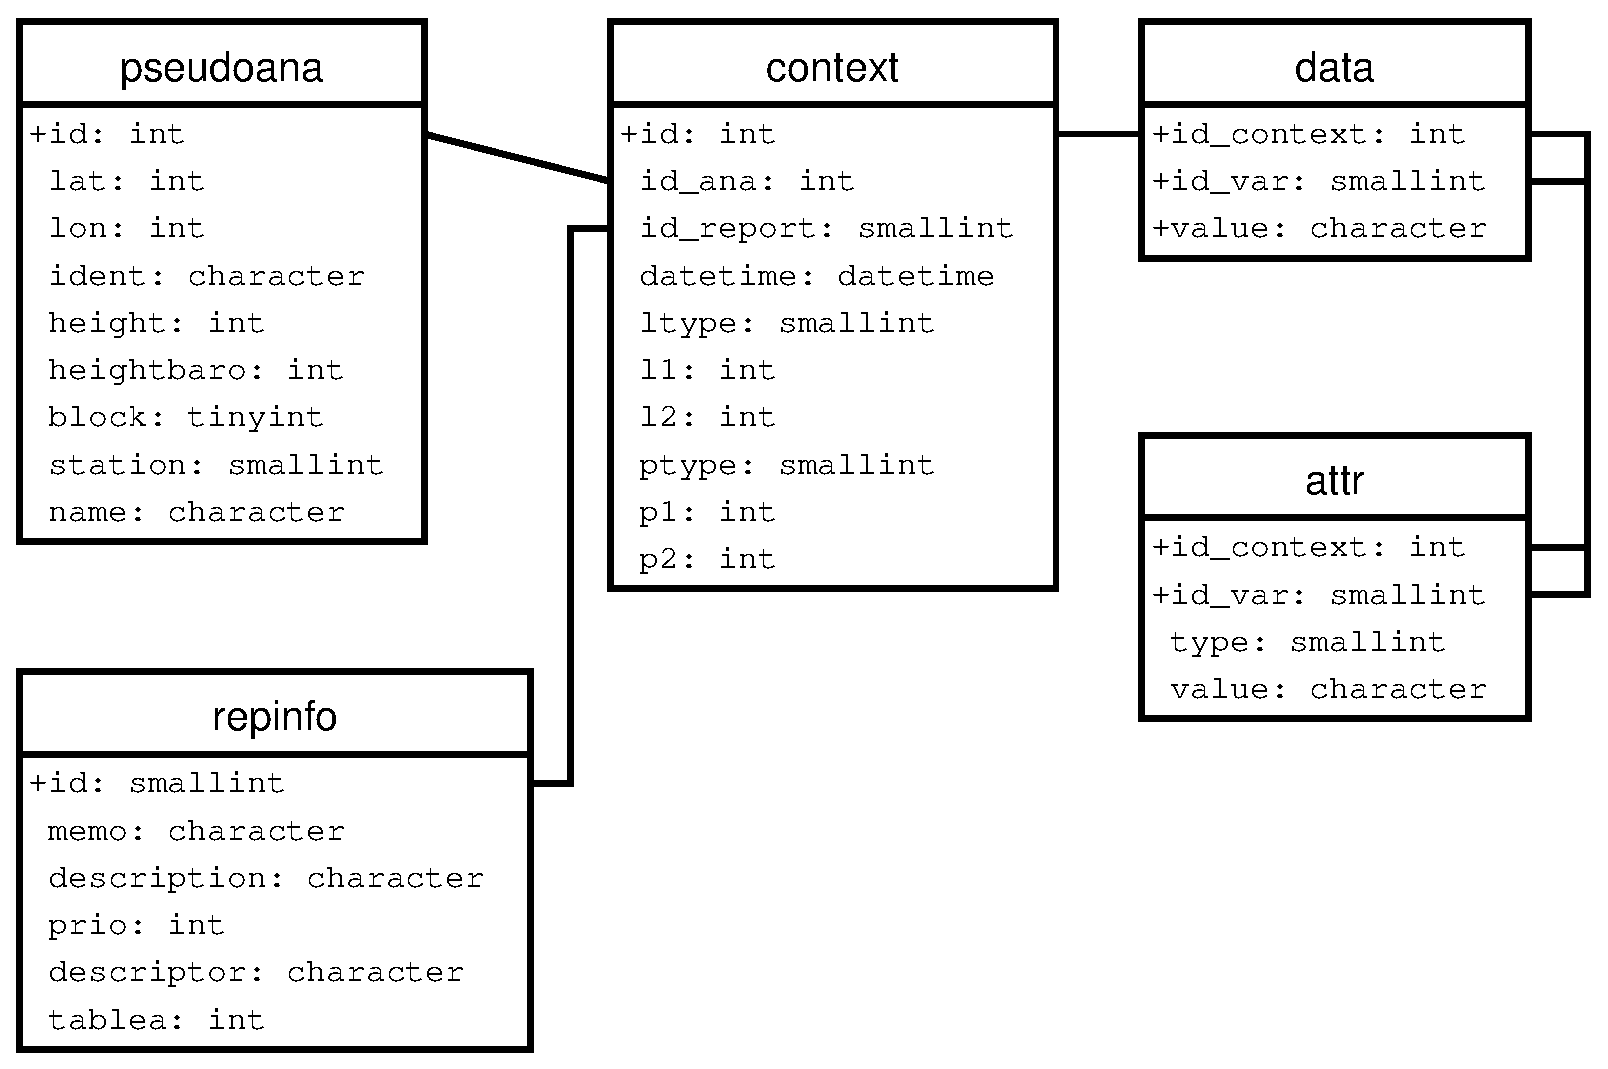
\includegraphics[width=\textwidth]{db.eps}
\end{center}
\caption{Structure of \dballe{} database}
\end{figure}

